
%%%%%%%%%%%%%%%%%%%%%%% file typeinst.tex %%%%%%%%%%%%%%%%%%%%%%%%%
%
% This is the LaTeX source for the instructions to authors using
% the LaTeX document class 'llncs.cls' for contributions to
% the Lecture Notes in Computer Sciences series.
% http://www.springer.com/lncs       Springer Heidelberg 2006/05/04
%
% It may be used as a template for your own input - copy it
% to a new file with a new name and use it as the basis
% for your article.
%
% NB: the document class 'llncs' has its own and detailed documentation, see
% ftp://ftp.springer.de/data/pubftp/pub/tex/latex/llncs/latex2e/llncsdoc.pdf
%
%%%%%%%%%%%%%%%%%%%%%%%%%%%%%%%%%%%%%%%%%%%%%%%%%%%%%%%%%%%%%%%%%%%


\documentclass[runningheads,a4paper]{llncs}
\usepackage{amssymb}
\usepackage{graphicx}
\usepackage{subfig}
\usepackage{amsfonts}

\usepackage{amssymb}
\usepackage{algorithm}
\usepackage{multirow}
\usepackage{amsmath}
\usepackage{array}
\usepackage{url}
\usepackage{amssymb}
\setcounter{tocdepth}{3}
\usepackage{geometry}%页面设置
\usepackage{graphics}%图片设置
\usepackage{caption}%注释设置



\usepackage{url}
\urldef{\mailsa}\path|{alfred.hofmann, ursula.barth, ingrid.haas, frank.holzwarth,|
\urldef{\mailsb}\path|anna.kramer, leonie.kunz, christine.reiss, nicole.sator,|
\urldef{\mailsc}\path|erika.siebert-cole, peter.strasser, lncs}@springer.com|
\newcommand{\keywords}[1]{\par\addvspace\baselineskip
\noindent\keywordname\enspace\ignorespaces#1}

\begin{document}

\mainmatter  % start of an individual contribution

% first the title is needed
\title{Probabilistic Topic and Role Model for Information Diffusion in Social Network}

% a short form should be given in case it is too long for the running head
%\titlerunning{Lecture Notes in Computer Science: Authors' Instructions}

% the name(s) of the author(s) follow(s) next
%
% NB: Chinese authors should write their first names(s) in front of
% their surnames. This ensures that the names appear correctly in
% the running heads and the author index.
%

\toctitle{Lecture Notes in Computer Science}
\tocauthor{Authors' Instructions}
\maketitle




\begin{abstract}
Information diffusion, which tackles the issue of how a piece of information spreads and reaches individuals in or between networks, has attracted considerable research efforts due to its widespread applications, such as viral marketing and rumor control. However, the process of information diffusion is complex and its underlying mechanism is still unclear. One important reason is that social influence takes many forms and each form may be determined by different factors. One of the biggest challenges is how to capture all the crucial factors of a social network such as users' interests (which can be represented as topics), users' attributes (which can be summarized as roles) and users' reposting behaviors in a unified manner to model the information diffusion process . Yet in the existing approaches concerning the social network analysis, these crucial factors are considered separately and processed independently. In this paper, we comprehensively investigate the high correlation and mutual influence between users' interests and roles in diffusion process, which are defined by the contents of the reposted messages and her structural properties, respectively. Then, a novel Topic and Role Model (TRM) is proposed, which integrates user topical interest extraction, role recognition and information diffusion modeling into a unified framework. We develop a Gibbs sampling based algorithm to estimate model parameters, and then fit the model to a large and real social network using historical information diffusion data. Experimental results show the validity and competitiveness of our model, compared to several state-of-the-art alternative models.

\keywords{user topic; user role; information diffusion ; social network}
\end{abstract}


\section{Introduction}

\emph{Information diffusion} focus on how a piece of information (knowledge) spreads and reaches individuals in or between networks~\cite{yang2015rain,xiong2012information}.
With the rapid development of online networks, such as Twitter, Facebook, Sina Weibo etc., it becomes easier for people to share or obtain the information they are interested in by posting or retweeting messages online~\cite{Abel2011Analyzing,Aslay2014Online,Yang2010Predicting}. Information on social media propagates more quickly than in real society~\cite{Gomez2012Inferring,Kwak2010What}. The process of the information diffusion is crucial for spreading technological innovations~\cite{tu2015prism}, word of mouth effects in marketing~\cite{Domingos2001Mining}, and opinion formulations~\cite{xu2012modeling}. In reality, the information diffusion process is complex, as is the influence of one user on another. Previous researches, such as \cite{Zhang2014Role,Chen2015Online,Tang2009Social} and empirical studies on online social networks, including Twitter~\cite{Grabowicz2016Distinguishing,Kwak2010What}, Facebook~\cite{Sekara2015Fundamental}, Sina Weibo~\cite{tu2015prism}, revealed many interesting phenomena and basic underlying laws. For example,in a social network,one user's final behavior decision is the balance between her own interests(which can be represented as topics) and her trusted friends with similar interests~\cite{Barbieri2012Topic,xu2012modeling,Zhang2014Role}. Users may have different attributes, for example, some users may be popular,and have many followers, but others may be different. How should we model the information diffusion process so that the model can capture the intrinsic relations between all these elements, such as individual attributes, users' topical interests and actions?


Information diffusion analysis has been attracting much interest from researchers. Some extensive efforts have been made in this field~\cite{xu2012modeling,Zhang2014Role}. From the perspective of structure of the network availability, information diffusion model can be classified into network structure based  methods and non-structure based methods. Non-structure based approaches are limited by the fact that they ignore the
topology of the network and only forecast the evolution of the rate at which information globally diffuses\cite{Aslay2014Online}.
In network structure based methods, there are two representative models, namely Independent Cascade(IC) model~\cite{Goldenberg2001Talk}and Linear Threshold model(LT) model~\cite{granovetter1978threshold}. They assume that the network structure determines the flow of information and focus on the structure of the process. Since these two models  require a diffusion probability between every two users, thus they have high computational complexity. To overcome this problem, ~\cite{Zhang2014Role,xu2012modeling} introduce the topic model such as LDA \cite{blei2003latent} to make users with same topic distribution share the same behavior pattern.
Zhang~\cite{Zhang2013Social} employed social influence locality  for modeling users' reposting behaviors by taking the phenomenon into consideration that users' behaviors are mainly influenced by close friends in their ego networks. Xu~\cite{xu2012modeling} assumed that the user posting behavior is mainly influenced by three factors: breaking news, posts from social friends and user's intrinsic interests. Tang~\cite{Tang2009Social} proposed a probabilistic factor graph model that takes the effects of user-to-user topic-wise influence strength for expert findings. Furthermore, topic-aware diffusion models assumed that either the topics associated with the diffusion process are specified in advance or independent with the user structural attributes~\cite{Chen2015Online}.

 Although much progress has been made, the results of existing work are not satisfactory, due to their limitations:

 \emph{1.} Most information diffusion models utilized only portions of the available social network information. For example, Zhang \cite{Zhang2013Social} only took the network structure information into consideration, ignoring the differences between the users themselves, such as user's preferences or interest, while \cite{xu2012modeling} assumed that breaking news, posts from social friends and user's interests influence user posting behaviors, ignoring the conformity influence in information diffusion.

 \emph{ 2.}The highly volatile user behaviors usually render it difficult to accurately uncover diffusion patterns for the approaches between individuals. For example, some users seem very active, and prefer to repost the messages from her idoles, while others may not.

  \emph{3.} The underlying mechanism of information diffusion is still unclear. One important reason is that social influence takes many forms and each form may be determined by different factors.

In reality, the information diffusion process is complex, as is the influence of one user on another. Social influence happens when one's opinions or behaviors are affected by others. It is well known that different types of social ties have essentially different influence on social actions.~\cite{Barbieri2012Topic,xu2012modeling,Zhang2014Role}claimed that one user's final behavior decision is the balance between her own interests(which can be represented as topics) and her trusted friends with similar interests. Obviously, users with similar preferences are more likely to be friends than others in social networks~\cite{wahba1973maslow,burt2009structural}. Topics are the collections of user's interests to post a message and provide the intentions for user's engagement in social networks~\cite{Pinto2014Modeling,xu2012modeling}. Moreover,the structure of the network affects how information may diffuse in a social network, in which the users' structural attributes determine their social roles in different communities~\cite{Wasserman1994Social,yang2015rain}. User's social role in turn affects the information diffusion process. For example, 1\% users with high Pagerank score \cite{page1999pagerank} acting as opinion leaders post 50\% URLs on Twitters information diffusion \cite{wu2011says}.

Consequently, we face some very interesting questions: Is there any dynamics or mutual influence between user interests and social roles? To what extent do they influence the information diffusion process? If, for instance, a famous artificial intelligent expert and a normal political-science major student both retweet the same two messages: one message about AlphaGO and the other one about the presidential candidate Trump, will the followers of each user retweet the two different messages equally? Specially, will the two users have the same influence strength on their common followers ? This paper offers a new perspective.

We introduce a TRM model to uncover and explore temporal diffusion. We model topics and roles in a unified latent framework, and extract role-aware topic level influence dynamics.  In this model, we group the users based on their structural properties and reposed information, and translate the calculations of individual level influence to the role-topic pairwise influence, which can provide a coarse-grained diffusion representation. These effective technologies facilitate our TRM model to accurately capture the backbone of information diffusion, as well as better predict and analyzes the diffusion.

Topics and social roles are both hidden. Pipeline approaches to extract these two factors in sequence fail to capture their interdependence. Though in recent years an array of techniques~\cite{yang2015rain,burt2009structural,Pinto2014Modeling,Zhang2014Role} have been developed for jointly leveraging these two critical factors, they all fall short of properly modeling the correlations between them. Besides the task of simultaneously extracting topics and social roles, we are even required to model the information diffusion process with temporal factors.

To tackle the above issues, this paper develops a latent model, TRM(Topic and Role Model), to extract topics, social roles and role aware topics dynamic in a unified way. We model topics and social roles as latent variables, and set up a generative process for observed network, contents of the reposted messages and time to accurately characterize the role-aware topic level information diffusion process.

Based on the extraction, we design an effective diffusion prediction method. Extensive experiments on large dataset show that our method greatly improves the prediction accuracy. To summarize, we make the following contributions:


\begin{itemize}
\item \textbf{Novel Perspective.} We systematically study on the building joint models to explore mutual influence for user topics and roles. It brings up a new into the information diffusion process. To the best of our knowledge, such a new angle has not been studied before.

  \item\textbf{Comprehensive Model.} We propose a latent model to uncover the hidden topics and roles as well as capture the information diffusion, which can model the process of information diffusion better than other models. We further devise a Gibbs sampler to estimate the parameters.

  \item \textbf{Inspiring Prediction \& Exploration} An effective diffusion prediction approach is developed which leverages the information diffusion patterns with user topics and social roles. We conduct extensive experiments to validate the proposed model over several baselines by employing two large real-world network as experimental datasets. Experimental result shows that the proposed model performs much better than the baseline methods.
\end{itemize}


\section{Related Work}

\textbf{Information diffusion.} Although online information diffusion has received increasing interest over the recent years ~\cite{yang2015rain,Goldenberg2001Talk,granovetter1978threshold,xu2012modeling}, modeling the diffusion in social networks remains an open problem.
Central to information diffusion is the estimation of influence strength. In representative information diffusion models, such as Independent Cascade(IC) model~\cite{Goldenberg2001Talk} and Linear Threshold model(LT) model~\cite{granovetter1978threshold}. Both types of models have the computational problem is that of selecting the set of initial users that are more likely to influence the largest number of users in the social network~\cite{Barbieri2012Topic}, and also have the over-fitting problem resulting from their large number of unknown parameters to learn. TRM addresses these two problems by allowing users with the same social role and user topical interests to share the same diffusion patterns, thus greatly reduce the number of parameters.
Social influence happens when one's opinions or behaviors are affected by others.

\textbf{Topic-aware influence.} While most of the above work utilizes the network structural and timing information to model the information diffusion process, a different line of work has considered analyzing the available textural information and use the latent topics of the messages as the user's needs or interests~\cite{xiong2012information,Pinto2014Modeling,Barbieri2012Topic}. Topics are the collections of user's interests to post a message and provide the intentions for user's engagement in social networks~\cite{Pinto2014Modeling,xu2012modeling}. Furthermore, users with similar preferences are more likely to be friends than others in social networks~\cite{wahba1973maslow,burt2009structural}.In~\cite{xiong2012information}, the authors assumed that the user's retweeting actions are mainly influenced by the three factors: breaking news, posts from social friends and user's intrinsic interest, and proposed a mixture latent topic model to predict the user's repost behaviors. In~\cite{Pinto2014Modeling}, the authors applied the Hawkes process to model the information diffusion process based on the latent topics of the user's. Most of the topic-aware information diffusion models take into considerations the topic of the user or the twitter, and neglect the user's structural attributes. In contrast to these models, we focus on the diffusion process not only with considering how the topical interests may influence such process, but also considering the different roles of users. Especially, the social role and user topical interest distributions of each user are not only determined by her structural attributes and the contents of the reposted messages respectively, but also by her diffusion behaviors.

\section{TRM diffusion model}
Online social networks, such as Twitter and Sina weibo, have become the central nexus for discussion of the topics of the day. On social networks, users from all over the world tweet or retweet a variety of topics of interests. Naturally, each user has distinct topical interests or personalized preference. To characterize the heterogeneity among all users, we model each user possesses a distinct probability that he or she is interested in retweetting messages. For example, consider a mini set of two topics: sports and movie. One may retweet the sports topic with a higher probability than the movie topic, while another user may be more interested in retweeting movie than retweeting sports. Given a set of topics, a user generates each word in their tweets from one of the topics based on the distribution specific to this topic. Moreover,the structure of the network affects how information may diffuse in a social network, in which the users' structural attributes determine their social roles in different communities~\cite{Wasserman1994Social}. It is well known that different types of social ties have essentially different influence on social actions. User's social role in turn affects the information diffusion process. For example, 1\% users with high Pagerank score \cite{page1999pagerank} acting as opinion leaders post 50\% URLs on Twitters information diffusion ~\cite{wu2011says}. Furthermore, social roles and diffusion are not independent of each other in nature. Intuitively, each user may play multiple roles with respect to different structural attributes, thus exhibiting different influential strengths in different diffusion process. For instance, one with high PageRank scores may act as opinion leader when she post on her area of expertise. To model the intuition that a user may take different social roles in different diffusion processes, we associate each user with a social role distribution.
  \begin{figure}[h]
\centering
\includegraphics[height=2.0in, width=2.5 in]{newmodel}
\caption{TRM model}
\label{fig:model}
\end{figure}

\subsection{Formulation}
Let $\mathbf{\emph{G = (V,E,X)}}$ where $V $ is the set of all the users and $E \subseteq V \times V $ is a set of relationships between users. Each factor ${e_i}_j =  < {v_i},{v_j} >  \in E$ represents user ${v_i} $ follows ${v_j} $, in other words, ${v_i}$ is the follower of ${v_j}$ and ${v_j}$ is the followee of ${v_i}$ in turn. Each user ${v_i} $ has $H$-dimensional attribute vector ${x_i} $, where $H$ is the number of all attributes. Each factor $ x_{vh} \subset X$ denotes the $h{\rm{ -th }}$ attribute of user $v$. We can define the user's attributes such as Pagerank Score~[\cite{page1999pagerank}], in degree and network  constraint score~[\cite{burt2009structural}], based on the structure of the social network. For each user $v \in V$, we use $N(v) = \{ u|u \in V,{e_{uv}} \in E\}$ to denote the set of followees of $v$. For a message, Whether a user activate her followers may also depend on the role she plays and the her intention she chooses.

To model the intuition that a user may have different interest topics and take different roles in information diffusion process, we associate each with an interest topic and social role distribution respectively:

\noindent\textbf{Definiton 1} \emph{\textbf{Topic distribution}}. In social networks, a user is usually interested in multiple topics. Formally, each user is associated with a vector ${\phi _v} \in {V^K}$, where $K$ is the number of topics($\sum\nolimits_k {{\phi _{vk}}}  = 1$).


\noindent\textbf{Definiton 2} \emph{\textbf{Role}}. Each user may play multiple different roles, denoted as $r = [1,2,...,R]$. Each role has a set of parameters for the distribution the attributes conform to. Here we use Gaussian distribution. If a user plays role $r$, its $h$-th attribute conforms to $({u_{rh}},{ \delta _{rh}}^{ - 1})$.

\noindent\textbf{Definition 3} \emph{\textbf{Role distribution}}. Each user has a multinomial distribution over roles, which is denoted as $\theta$.  \textbf{${\theta _v}$} denotes the probability for user $v$ to play role $r$, and is subject to ${\sum\nolimits_r \theta  _{vr}} = 1$.

\noindent\textbf{Definition 4} \emph{\textbf{Topic-Role Pair}}. Whether a user $v$ would repost a message posted by her followee $u$ depends on the $u's$ role she plays and the topic she chooses. We use $\rho $ to denote the distribution of topic-role pairs over reposting actions.
In information diffusion process, the actions of reposting messages only contains two cases, so we can use a Bernoulli distribution to model the distribution of topic-role pairs over actions. In other words, $\rho_rk $ denotes the influence strength that a user plays role $r$ and chooses the topic $k$ to successfully activate one her follower for a message.
\vspace{-15pt}


\begin{table}[h]
\centering
\caption{Notations}
  \begin{tabular}{p{2.5cm}<{\centering}|p{9.5cm}<{\centering}}
%\begin{tabular}{|c|c|}

  \hline
  % after \\: \hline or \cline{col1-col2} \cline{col3-col4} ...
 \bfseries SYMBOL & \bfseries DESCRIPTION  \\
\hline
$R,K,H,W$     & number of social roles,topics,attributes and unique words in the dataset\\
\hline

$T$ & the largest timestamp in a given diffusion model\\
\hline

$N_d$ & the number of words in the $d$th messages\\
\hline

$e_{iuv}^t$  & a latent variable denoting whether user $v$ reposts the message $i$ posted by user $u$ at time $t$\\
\hline
$k_{d}$  & topic associated with post $d$ \\
\hline
${\phi _v}$ & Multinomial distribution over topics specific to user $v$\\
\hline
${\psi _k}$ & Multinomial distribution over words specific to topic $k$ \\
\hline

${\theta _v}$ & Multinomial distribution over roles specific to user $v$\\
\hline
${\lambda _r}$ &  geometric distribution over $\Delta t$ associate with role $r$\\
\hline
${\rho _{rk}}$ &Bernoulli distribution over decision to repost a message associate with topic $k$ and role $r$\\
\hline
${u_{rh}}$  &mean of  $h$-th attribute specific to role $r$\\
\hline
${\delta _{rh}}$ & standard deviation of $h$-th attribute  specific to role $r$ \\
  \hline
\end{tabular}
 \label{notations}

\end{table}

\subsection{Model description}
Based on the above definitions, we explain the proposed TRM model. Our goal is to devise a probabilistic generative model for extracting the user topical interests, learning user social roles and modeling information diffusion simultaneously. Fig.(\ref{fig:model}) illustrates the model, where $f$ is a diffusion function. TRM determines user topical interests of each user according to both her reposted messages and her behaviors in diffusion process. The basic idea is that the user's actions of reposting messages not only depend on the social role she plays, but also depend on her topical interests. We use the content of user's reposted messages to determine her topic distribution and use user's attributes to determine her role distribution, which are all then used as priors to guide the sampling for user's actions. Overall, the TRM model we proposed consists of three parts: the user's messages generation ,the user's attributes generation and modeling the information diffusion process.

\subsubsection{User's messages generation}
Here, we associate a single hidden variable with each message to indicate its topic due to the limitations of the length of characters in a single message. The generative process of the message $d$ posted by user $v$ can be described as follows:

1. Draw a ${\phi _v}$ from from Dirichlet (${\pi}$)

2. Draw a topic $k$ from multinomial distribution ${\phi _v}$

3. Draw a ${\psi _k}$ from Dirichlet (${\varepsilon}$)

4. For each word $n=1,...,{N_d}$, draw a word ${w_{dn}}$ from mulitnomial distribution ${\psi _k}$.


\subsubsection{\textbf{Social attributes generation}}
Each user may play several roles in different information diffusion processes and is subject to a certain distribution over attributes, denoted by $\theta _v$. Each user is a random mixture over roles and can be denoted by $ v = ({x_1}...{x_h}...{x_H})$. For each individual attribute of user $v$, we first generate $v's$ role distribution ${\theta _v}$, then generate a latent role $r$ from user $v$'s role distribution ${\theta _v}$, next draw the value of attribute $h$ from the normal distribution $({u_{rh}},{ \delta _{rh}}^{ - 1})$.
\emph{}The generative process of the value of attribute $h$ for user $v$ in a social network can be described as follows:

1.Draw a ${\theta _v}$ from Dirichlet $(\alpha)$

2.Draw a role $r$  from multinomial distribution $ {\theta _v}$.

3.Draw the value of attribute $h$ over role $r$: ${x_{rh}}$ $\sim $ $({u_{rh}},{\delta _{rh}}^{ - 1})$


\subsubsection{\textbf{Model information diffusion process}}
Inspired by our exploratory analysis, which reveals that topical interests and social roles of a user affect the information diffusion process. Specially, we incorporate the user topics and roles in the information diffusion process. We introduce topic-role parameters ${\rho _{rk}}$ denotes the probability that one user plays role $r$ successfully activate another user specific to topic $k$ and a per-role parameters ${\lambda _r}$ denotes the probability that cause a 1-timestamp delay in information diffusion. At anytime, user $v$ will become active at least one of her followees activate her successfully. We use Independent Cascade Model as diffusion function $f$ in TRM model.

More specifically, we first generate the influence strength and diffusion delay corresponding to ${\rho _{rk}}$ and ${\lambda _r}$, respectively.
Consider a message $i$ posted by user $u$ at time $t$, $u$ will have only one chance to activate her follower $v$. Firstly, user $u$ draws role $r$ she will play from role distribution ${\theta _{u}}$. Next, draws the topic $k$ the message will be interested in for $u's$ follower $u$ from multinomial distribution ${\phi _u}$, and then generate a time delay $\Delta t$  from  geometric distribution ${\lambda _r}$. At time $t' = t + \Delta t + 1$, we draw the $e_{iuv}^t$ from Bernoulli(${\rho _{rk}}$) to determine whether user $u$ will succeed in activating user $v$.

For each action of repost :

1. Draw a role $r$ from  multinomial distribution ${\theta _{u}}$.

2. Draw the topic $k$ from multinomial distribution ${\phi _u}$.

3. Draw ${\rho _{rk}}$ from beta($\beta$) prior.

4. Draw the ${\lambda _r}$ from beta($\eta$).

6. Draw $\Delta t$ from geometric distribution ${\lambda _r}$.

7. Toss a coin, draw the $e_{iuv}^t$ from Bernoulli(${\rho _{rk}}$).

\subsection{Model Learning}
Learning the model is to find a configuration for the parameters $\{ \theta ,\phi ,\rho ,\lambda \}$ to maximizes the log-likelihood objective function.
The posterior probability of ${k_{d}}$, which denotes that the latent topic $k$ for the post $d$ of user $u$ to activate her follower is calculated by:
\begin{equation}\label{14}
%\setlength{\abovedisplayskip}{3pt}
  p(k_d=k|{k_{{}^ - ud}}) = \frac{{{n_{ - uk}} + \pi }}{{\sum\limits_k {({n_{ - uk}} + \pi )} }} \times \prod\limits_{n = 1}^{{N_d}} {(\frac{{n_{_{{w_{dn}}}}^k + \beta }}{{\sum\limits_w {(n_{_w}^k + \beta )} }})}
 % \setlength{\belowdisplayskip}{4pt}
\end{equation}
where the counter $n_{uk}$ denotes the number of times topic $k$ being sampled with user $u$; $w_{dn}$ means the $n$-th word in post $d$ and $n_w^k$ denotes the number of times word $w$ being assigned to topic $k$. The superscript$- uk$ on the counters indicates exclusion of the current observation(resp.the message $d$ posted by user $u$) from the counts.

According to [\cite{bernardo2009bayesian}] ,we adopt :
\begin{equation}\label{10}
\begin{split}
&{u_{rh}} \approx E({u_{rh}}) = \frac{{{\tau _0}{\tau _1} + {n_{rh}}{{\overline x }_{_{rh}}}}}{{{\tau _1} + {n_{rh}}}}\\
& {\delta _{rh}} \approx E({\delta _{rh}}){\rm{ = }}\frac{{{\rm{2}}{\tau _2}{\rm{ + }}{n_{rh}}}}{{{\rm{2}}{\tau _3}{\rm{ + }}{n_{rh}}{s_{rh}} + \frac{{{\tau _1}{n_{rh}}{{({{\overline x }_{_{{r_{}}h}}} - {\tau _0})}^2}}}{{{\tau _1} + {n_{rh}}}}}}
\end{split}
.\end{equation}


Similarily, after Gibbs sampling, parameters $\{ \theta ,\phi ,\rho ,\lambda \}$ can be estimated by:

\begin{equation}\label{12}
\begin{split}
{\theta _{ur}}  = \frac{{{n_{ur}} + \alpha }}{{\sum\limits_r {({n_{ur}} + \alpha )} }}
~~~{\phi _{uk}}  = \frac{{{n_{uk}} + \pi }}{{\sum\limits_k {({n_{uk}} + \pi )} }}\\
{\rho _{rk}}= \frac{{{n_{erk(e = 1)}} + {\beta _1}}}{{{n_{0rk}} + {\beta _0} + {n_{1rk}} + {\beta _1}}}
~~~{\lambda _r}  = \frac{{{n_r} + {\eta _1}}}{{{s_r} + {\eta _0} + {\eta _1}}}
\end{split}
.\end{equation}

where $\overline r ,\overline k,\overline {\Delta t},\overline e$ respectively represent a new observation of $r,k,\Delta t $ and $e$.



\section{Experiment}
\subsection{Experimental setup}


We evaluate the effectiveness of the proposed model on two real-world datasets belonging two different social networks:


 \noindent$\bullet$\textbf{Weibo} is a dataset from Sina Weibo Website, the largest microblogging service in China. The Weibo data we used in our experiment is from \cite{tu2015prism} with 66,348 users, 13,487,120 repost actions. We select the original posts that were reposted by larger than 6 users, and use remaining 129,560 original posts for experiments. For a given twitter from a user, we would like to predict who will repost the twitter.

 \noindent$\bullet$\textbf{Citation Network Database(CND)}\cite{Zhang2014Role} is extracted from DBLP, ACM, MicroSoft Academic Graph, and other sources. We select the original paper that were citated by larger than 6 users, and use remaining 67,414 original papers for experiments. For a given paper, we would like to predict which author will cite this paper next.

Since the retweet or cite action prediction is much similar a ranking problem, we prefer the precision at top ranked results as the evaluations of our proposed model. Specially, given a message or a paper $i$ produced by user $v$, we calculate the retweet or cite probability of each $v's$ followers, and we use P@10(Precision of top-10 predictions), P@50, P@100, and MAP(Mean Average Precision) to evaluate the ranking prediction results for each message and aggregate the results for all messages together.

We compare TRM with several representative methods for user's  prediction Count, LDA \cite{blei2003latent}, MUPB \cite{xu2012modeling},Social Role-Aware Information Model(Rain) \cite{yang2015rain}.


\noindent$\bullet$\textbf{Count}\textbf{:} In Count, the probability of a user reposting a message is in direct proportion to the number of followees who have reposted message $i$. This method assumes that a user's reposting decision only depends on her followees.

\noindent$\bullet$\textbf{LDA}\textbf{:} In LDA~\cite{blei2003latent}, the probability of a user reposting a message based on the topic distributions of  message $i$ and $v$'s all reposted posts in the training data set. This method only takes contents of the messages into account, and ignores the whole and local social network structural attributes.

\noindent$\bullet$\textbf{MUPB}\textbf{:} MUPB~\cite{xu2012modeling} assumed that the user posting behavior is mainly influenced by three factors: breaking news, posts from social friends and user's intrinsic interests. Although this method can to some extent help extract the topics of users, however, it failed to capture the real motivation of users to publish content, as user behavior can easily affected by the structure of the network, other than user interest.

\noindent$\bullet$\textbf{Rain}\textbf{:} Rain~\cite{yang2015rain} predicts whether user $v$ will repost message $i$ based on the user $v's$ role distribution and the information diffusion attributes corresponding to each role. This method ignored the user's intrinsic interests satisfactions by reposting the message $i$.


\noindent$\bullet$\textbf{TRM}\textbf{:} This is the proposed method.
We empirically set the model parameters as $R=10,K=10,\alpha {\rm{ = }}0.1,\pi {\rm{ = }}0.1 ,\varepsilon {\rm{ = }}0.1$
$\beta  = (1,1),\eta  = (1,1)$

\vspace{-20pt}
\begin{table}[h]
\centering
\caption{Performance comparison on two datasets evaluated by Precision@n and MAP.}
  \begin{tabular}{p{1.5cm}<{\centering}|p{1.2cm}<{\centering}p{1.2cm}<{\centering}p{1.2cm}<{\centering}p{1.2cm}<{\centering}|p{1.2cm}<{\centering}p{1.2cm}<{\centering}p{1.2cm}<{\centering}p{1.2cm}<{\centering}p{1.2cm}<{\centering}}
%\begin{tabular}{|c|c|}
\hline
\hline
\multicolumn{5}{c|}{Weibo}  & \multicolumn{4}{c}{CND} \\
\hline

  % after \\: \hline or \cline{col1-col2} \cline{col3-col4} ...
 Method &  P@10&  P@50& P@100& MAP & P@10&  P@50& P@100& MAP \\
\hline

 Count     & 0.007 &0.006 &0.006   &0.013  &0.089 & 0.029 &0.017  &0.127\\
\hline
 LDA     & 0.112 &0.039 &0.020   &0.085  &0.153 &0.049 & \textbf{0.030} &0.198\\
\hline
 MUPB     & 0.405 &0.137 &0.079   &0.415   &0.122&0.038&0.022 &0.307\\
\hline
 Rain     & 0.407 &0.146 &0.083   &0.427  &0.121 &0.038 &0.021 &0.299\\
\hline
TRM     &\textbf{ 0.429} &\textbf{0.156} &\textbf{0.088}   &\textbf{0.458} &\textbf{ 0.143} &\textbf{0.043} &0.024   &\textbf{0.345}\\
 \hline
\end{tabular}
 \label{results}
\vspace{-10pt}
\end{table}


\subsection{Experimental Results}
\begin{figure*}[ht]
\centering
\subfloat[Weibo] {\includegraphics[width=0.40\textwidth,height=1.8in]{weibo_rain.eps}
\label{fig:2a}}
\hspace{5mm}
{\includegraphics[width=0.40\textwidth,height=1.8in]{weibo_mupb.eps}
\label{fig:2b}}
\hspace{5mm}
%\hspace{5mm}

\centering
\subfloat[CND] {\includegraphics[width=0.4\textwidth,height=1.5in]{citation_rain.eps}
\label{fig:2c}}
\hspace{5mm}
{\includegraphics[width=0.4\textwidth,height=1.5in]{citation_mupb.eps}
\label{fig:2d}}
\hspace{5mm}



\caption{Effect of Mutual Influence: the contribution of topic and roles on repost prediction.}\label{fig2}
\end{figure*}



\textbf{Better Performance.} The performance comparison on the two datasets evaluated by P@10, P@50, P@100 and MAP is illustrated in Table \ref{results}. We can discover that TRM model clearly outperforms Count, LDA, MUPB, and Rain nearly on all metrics in Weibo (+0.076- 0.445 improvement in terms of average MAP) and CND(+0.049-0.218 improvement in terms of average MAP). Due to the lack of supervised information, Count performs worst on both datasets. Whereas, the Count and LDA model outperform better in CND than Weibo. Since a author usually only focuses one or two  fields of study, thus the users in CND database usually cite the papers with the similar topics. The Count and LDA model all ignore the user's social structural attributes. Prediction of the user's reposts action based on LDA only depends on the user's history reposts, and ignores the situation where a user needs or topic distributions may change over time. TRM also outperforms MUPB and Rain on all metrics. Although MUPB and Rain also considers user topics and social roles, respectively, they still ignores the correlations and mutual influence between topics and roles.
%\vspace{-20pt}

%\vspace{-30pt}


%\vspace{-15pt}

\noindent\textbf{Effect of Mutual Influence.} We also examined the nature and the effectiveness of the associated latent factors on the mutual , and Fig.(\ref{fig2}) demonstrates their feasibility in our modeling. Note that if we do not incorporate the latent role or topic factor, our TRM model becomes the traditional MUPB or Rain approach, respectively. It shows that the latent factors consistently enhance the precision(evaluated by P@10,P@50 and MAP)for the repost prediction. For example, the latent topic and role factor significantly improve the MAP by 3.1\%(from 42.7\% to 45.8\%), and improve the MAP by 4.3\%( from 41.5\% to 45.8\%) for the repost prediction, respectively. These results also illustrate that the user's topics and social roles are very crucial to model the information diffusion.
%\vspace{-15pt}

\begin{figure*}[htp]
\centering
\subfloat[Weibo] {\includegraphics[width=0.25\textwidth,height=1.5in]{weibo_PR.eps}
\label{fig:3a}}
\hspace{5mm}
 {\includegraphics[width=0.25\textwidth,height=1.5in]{weibo_CS.eps}
\label{fig:3b}}
\hspace{5mm}
{\includegraphics[width=0.25\textwidth,height=1.5in]{weibo_PRCS.eps}
\label{fig:3b}}
%\hspace{5mm}
\centering
\subfloat[CND] {\includegraphics[width=0.25\textwidth,height=1.5in]{citation_PR.eps}
\label{fig:3b}}
\hspace{5mm}
{\includegraphics[width=0.25\textwidth,height=1.5in]{citation_CS.eps}
\label{fig:3b}}
\hspace{5mm}
{\includegraphics[width=0.25\textwidth,height=1.5in]{citation_PRCS.eps}
\label{fig:3b}}
\caption{Role analysis on two datasets: the correlation of influence strength with\emph{ Pagerank Score, Network Constraint Score and Pagerank/Network Constraint Score}}\label{fig3}
\end{figure*}




\noindent\textbf{Social role analysis.} The learned parameters $\rho$ represent the influence strength of a user for different topics and roles. The method also learns ${u_{rh}}$, which denotes the mean value of social attribute $k$ for role $r$, and ${\rho _{rk}}$ denotes the topic-role pair activate probability of topic $k$ for role $r$. So we can use the $P({r}) = \sum\nolimits_k {{\rho _{rk}}}$ to denotes the influence strength for role $r$.
Fig.(\ref{fig3}) shows the correlations between a role's social attribute and its influence strength. We discover that the correlation follows a logarithm function. We try different forms of functions to fit the remaining data points and select logarithm function of $R^2$. When fitting the data points, we first remove the roles with a small number of related users. As Fig.(3a), Fig.(3b) show that people who have larger Pagerank score or smaller
Network constraint score will have greater influence in the information diffusion process than ordinary people. This can be explained that people with larger Pagerank score tend to have more followers, and her posted messages will be more likely to be reposted. And people with smaller network constrain score tend to be a structural hole to connect two or more communities, and her posted messages will more easily be propagated to different social network communities.


\begin{figure*}[ht]
\centering
\subfloat[Weibo] {\includegraphics[width=0.4\textwidth,height=2.0in]{weibo_entropy.eps}
\label{fig:4a}}
\hspace{5mm}
\hfil
\subfloat[CND] {\includegraphics[width=0.4\textwidth,height=2.0in]{citation_Entropy.eps}
\label{fig:4b}}
\hfil
\\
\caption{The average entropy of topical distributions for each role on two datasets.}\label{fig:4}
\end{figure*}
\noindent\textbf{Correlation between user topic and social role.}
We further study the correlation between user topic and social role. To conduct this experiment, we first analyze estimated Gaussian parameters of TRM to uncover the meaning of the latent roles learned by TRM. Inspired by the work of~\cite{page1999pagerank,burt2009structural,Zhang2014Role,yang2015rain}], we group users into opinion leader, structural hole spanners and ordinary users. For instance, a latent role with small network constraint score is considered to be representing the structural hole spanners. Furthermore, the learned parameter $\phi$ represent the topic distribution for different users. Inspired by~\cite{Grabowicz2016Distinguishing}, we compute the entropy of user's topical distributions to measure how much topical a user's interests or topics are.
For a user $v$, the entropy of her topical interests distribution is computed as follows: $Hp(v) =  - \sum\limits_k^K {{\phi _{vk}}\log (} {\phi _{vk}})$.
To further analysis the correlations between users' topics and roles, we continue to calculate the average entropy for each role as follows:$Hp(r) =  \frac{1}{{\left| {{N_r}} \right|}}\sum\limits_{v \in {A_r}}^{} {Hp(v)}$,
where $A_r$ denotes the set of users to be assigned to role $r$, $N_r$ denotes the number of users in $A_r$. The higher the entropy, the less topical the role are.
 Fig.(\ref{fig:4}) demonstrates the correlations between user topics and roles. The higher the entropy, the less topical the role are. It follows that the most topical would be a user that is interested in only a single topic, whereas the least topical would be a user is interested in all topics with equally preferences. Thus the phenomenon in Fig.(\ref{fig:4}) may be explained as follows: most of opinion leaders post the messages about their areas of expertise and they tend to focus on regional and specialized topics, the structural spanners have broad interests than opinion leaders since they usually focus on more general topics which tend to propagate from one community to another more easily, the ordinary users have more broad interests since they behave more randomly. In Fig.(\ref{fig:4b}), the structural spanner has higher entropy value than ordinary users. The phenomenon may be explained as: when a person have published lots of papers in different regions, she may become more open-minded and tend to accept new ideas from others.

%\vspace{-10pt}
\section{Conclusions}
\vspace{-10pt}
In this paper, we study how to model the information diffusion process by capturing the user topics and social roles. We devise a probabilistic generative model framework, TRM to extract the user topics, recognize the social roles and model information diffusion. Our model allows for mining the correlations between users' topics and roles. Our experiments on a real social network data set show some interesting results that opinion leader tend to be more topical than the other roles, and the structural hole spanners tend to focus on more general topics. In addition, our method also outperform state-of-art baselines on the task of repost prediction in a large real social network.



{

\bibliographystyle{abbrv}
\bibliography{Myinstruct}
}
\end{document}
